% coding:utf-8

%----------------------------------------
%FOSADSVB, a LaTeX-Code for a summary of digital signal processing
%Copyright (C) 2015, Mario Felder & Michi Fallegger

%This program is free software; you can redistribute it and/or
%modify it under the terms of the GNU General Public License
%as published by the Free Software Foundation; either version 2
%of the License, or (at your option) any later version.

%This program is distributed in the hope that it will be useful,
%but WITHOUT ANY WARRANTY; without even the implied warranty of
%MERCHANTABILITY or FITNESS FOR A PARTICULAR PURPOSE.  See the
%GNU General Public License for more details.
%----------------------------------------

\chapter{Zufallssignale}
Stochastische Prozesse in Kombination mit LTI Systemen sind wichtige Werkzeuge zur Modellierung 
von Zufallssignalen. Sie sind besonders wichtig in der Audio- und Kommunikationstechnik.
\section{Autokorrelation und Spektrum}
\subsection{Betrachtung im Zeitbereich}
Mittelwert eines Zufallssignals $x[n]$:
\[ m_x = E\{x[n]\} \]
Autokorrelation eines Zufallssignals $x[n]$:
\[ \gamma_{xx}[m] = E\{x^*[n] \cdot x[n+m]\} \]
Wobei $\gamma_{xx}[0]$ die Leistung $P_x$ repräsentiert.\\
Die Autokorrelation ist gespiegelt symmetrisch an der y-Achse. Für Zufallssignale gilt:
\[ \gamma_{xx}[m] = \gamma_{xx}^*[-m] \]
Signale, welche den Mittelwert nicht bei Null haben, werden teils mit der Autokovarianz
statt der Autokorrelation charakterisiert:
\[ c_{xx} = E\{ (x[n]-m_x)^*\cdot(x[n+m]-m_x) \} \]
\[ y_{xx} = c_{xx}[m] + _x^2 \]
Die Autokovarianz bei $m=0$ repräsentiert die Varianz:
\[ E\{|x[n]-m_x|^2\} \]
\subsection{Betrachtung im Frequenzbereich}
Zufallssignale weisen eine nicht endliche Energie auf, es existiert also keine Fouriertransformierte.
Es kann jedoch ein Interval $[n_1,n_2]$ mit der DTFT betrachtet werden.
Spektrum durch die DTFT im Intervall $[n_1,n_2]$:
\[ X_{[n_1,n_2]}(\Omega) = \sum_{n=n_1}^{n_2}x[n]\cdot e^{-j\Omega n} \]
Das \textbf{Leistungsdichte-Spektrum} (power density spectrum) ergibt sich aus der 
DFT der Autokorrelationssequenz:
\[ \Gamma_{xx}(\Omega) = \sum_{m=-\infty}^{\infty}\gamma_{xx}[m] \cdot
	e^{-j\Omega m} \]
Die Leistung lässt sich durch Integration über 	$\Gamma_{xx}(\Omega)$ oder $\gamma_{xx}[0]$ ermitteln.
Bei realen Signalen ist die Form "'gerade"' (gespiegelt an der y-Achse). Es reicht also für reale Signale,
im Bereich $\Omega = [0,\pi]$ zu berechnen.
\[ P_x = \frac{1}{2} \int_{-\pi}^{\pi} \Gamma_{xx}(\Omega) \text{d} \Omega \qquad \qquad  \text{oder}
		\qquad \qquad	P_x = \gamma_{xx}[0] \]
Die Autokorrelation und das Leistungsdichte-Spektrum enthalten also die selben Informationen.
Aufgrund der fehlenden Phaseninformation ist es jedoch nicht möglich, $x[n]$ aus $\Gamma_{xx}(\Omega)$
oder $\gamma_{xx}[m]$ zu rekonstruieren.
~\\\\
\textbf{Weisses Rauschen:}\\
Aufeinander folgende Samples sind vollständig unkorreliert, das 
Leistungsdichte-Spektrum ist über $\Omega$ konstant. Es beinhaltet alle Frequenzen mit uniformer
Verteilung. Die Autokorrelation lautet:
\[ \gamma_{ww}[m] = \left\lbrace\begin{matrix}
	\sigma_w^2	& \textrm{if } m = 0\\
	0			& \textrm{if } m \neq 0
\end{matrix}\right. \]
Im folgenden werden zwei unterschiedliche Signale miteinander verglichen. Besonders die 
Grössenordnungen der x-Achsen bei der Autokorrelation und des Spektrums sind interessant. 
\begin{center}
	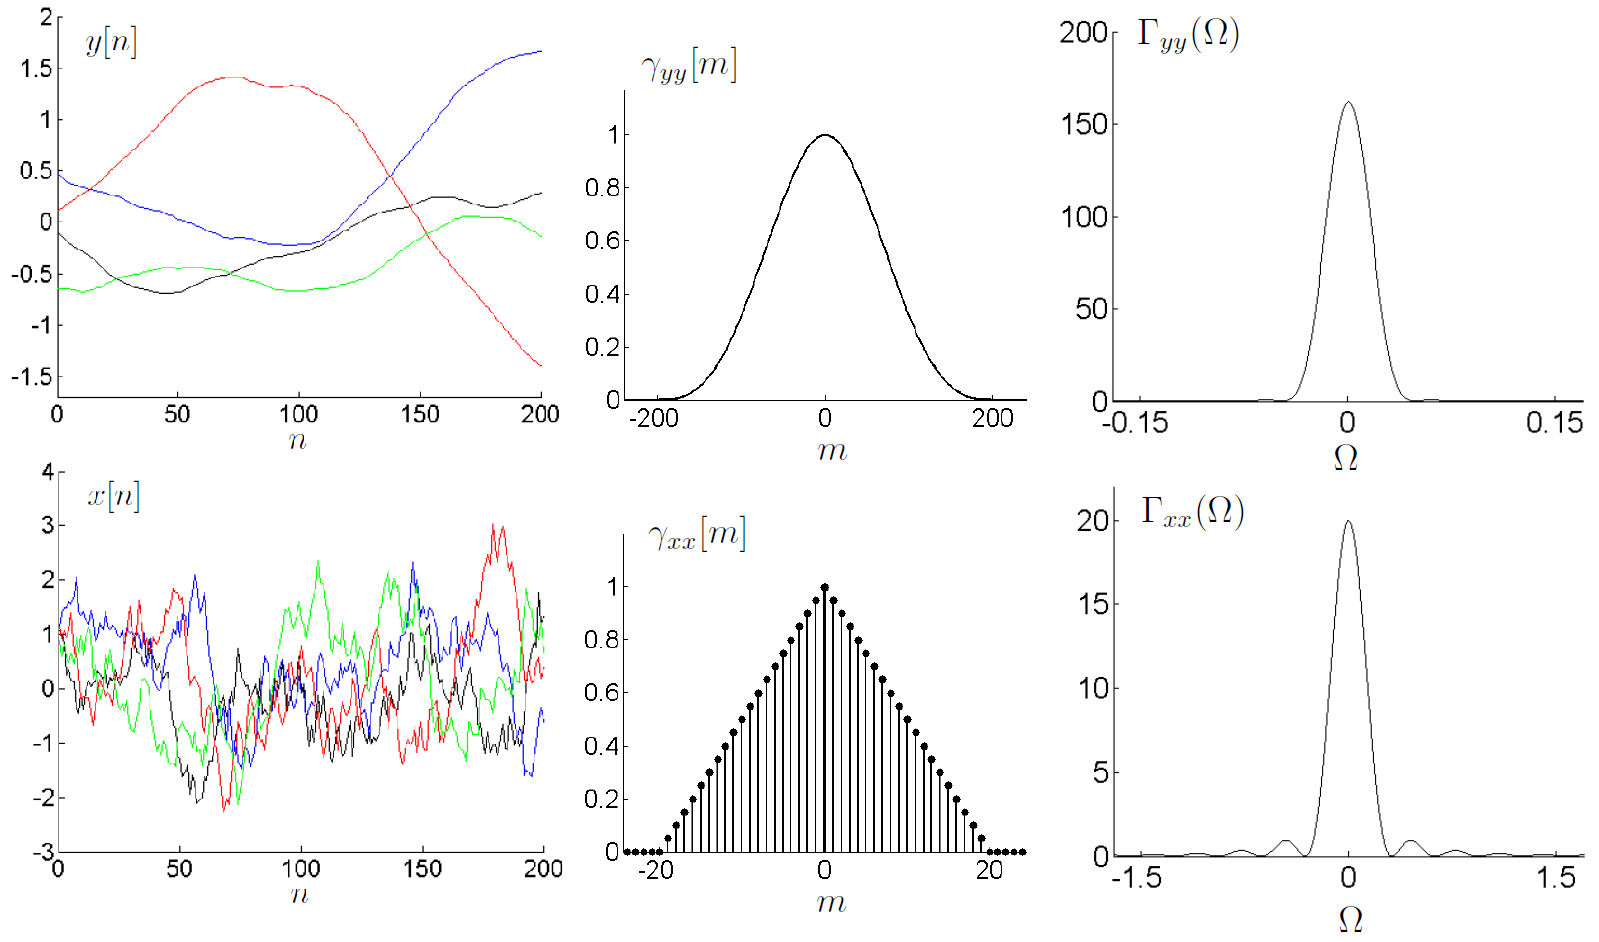
\includegraphics[width=0.8\textwidth]{../fig/vergleich_zufallssignale}
\end{center}

%===============================================================================
\section{Spectral Shaping durch LTI Systeme}
Mittelwert des Ausgangssignals $y[n]$ nach einem LTI-System $H$:
\[ E\{y[n]\} = m_y = m_x \cdot \sum_{k=-\infty}^{\infty} h[k] = H(0) \cdot m_x \]
, da der Frequenzgang gegeben ist als: 
\[ H(\Omega) = \sum_{k=-\infty}^{\infty}h[k]\cdot e^{-j \Omega k} \]
Autokorrelation von $y[n]$ ($i$ geht wie $k$ von $-\infty$ bis $\infty$):
\[ \gamma_{yy}[m] = h^*[-i]*\gamma_{xx}[m]*h[k] \]
Aus der erhaltenen Formel für Mittelwert und der Autokorrelation lässt sich folgende Aussage treffen:\\
\hspace{10mm} \textrightarrow Der Ausgang eines LTI-Systems mit stationärem Zufallssignal am Eingang ist erneut stationär.\\\\
Leistungsdichte-Spektrum am Ausgang:
\[ \Gamma_{yy}(\Omega) = H^*(\Omega)\cdot\Gamma_{xx}(\Omega)\cdot H(\Omega) 
	= |H(\Omega)|^2 \cdot \Gamma_{xx}(\Omega) \]

	 
%===============================================================================
\section{Lineare Modelle für Stochastische Prozesse}
\subsection{Filtern von White Noise}
Ein Whitenoise-Signal $w[n]$ durchläuft ein LTI-System. Am Ausgang entsteht 
farbiges Rauschen. 
\begin{center}
	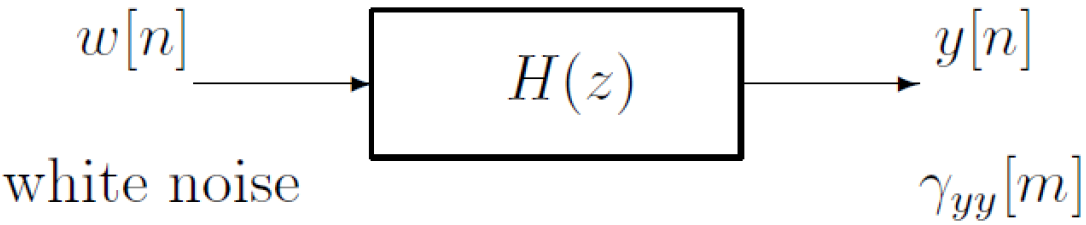
\includegraphics[width=0.35\textwidth]{../fig/filtering_of_white_noise}
\end{center}
Die $z$-transformierte der Autokorrelations-Sequenz für Ein- und Ausgang des Systems lauten:
\[ \Gamma_{ww}(z) = \sigma_w^2 \qquad \qquad \text{sowie} \qquad \qquad 
	 \Gamma_{yy}(z) = H(z^{-1})\cdot \Gamma_{ww}(z) \cdot H(z) \]
Angenommen, ein Zufallssignal mit einem Spektrum sei gegeben, und das Filter $H(z)$
sei gesucht. Es gilt für die Übertragungsfunktion:
\[ H(z) = \frac{B(z)}{A(z)} = \frac{\sum_{k=0}^{M} b_{k} \cdot z^{-k}}
								{1+ \sum_{k=1}^{N} a_{k} \cdot z^{-k}} \]
Die Null- und Polstellen von $A(z)$ und $B(z)$ seien alle
im Einheitskreis, das System $H(z)$ demnach kausal und stabil.
Ausgang des LTI:
\[ \Gamma_{yy}(z) = \sigma_w^2 \cdot H(z) \cdot H(z^{-1}) =
  \sigma_w^2 \cdot \frac{B(z) \cdot B(z^{-1})}{A(z) \cdot A(z^{-1})} \]
\subsection{Noise Whitening}
In diesem Fall wird stationäres Zufallsrauschen in weisses Rauschen umgewandelt. 
\begin{center}
	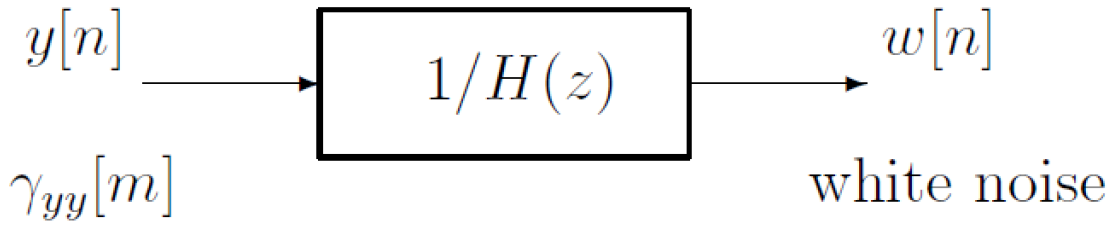
\includegraphics[width=0.35\textwidth]{../fig/noise_whitening}
\end{center}
Der Filter kann umgesetzt werden, indem die inverse Übertragungsfunktion $\frac{1}{H(z)}$ 
angewendet wird.\\\\
Für das Ausgangssignal des Noise Whitening Filters ergibt sich:
\[ w[n] = \frac{1}{b_0}\left( y[n] + \sum_{k=1}^{N}a_k\cdot y[n-k] - 
	\sum_{k=1}^{M}b_k\cdot w[n-k] \right) \]
	
%===============================================================================
\subsection{Moving average model (MA)}
$H(z)$ ist ein FIR-Filter mit Ordnung $M$ welcher ein weisses Rauschen $w[n]$
in ein Zufallssignal transformiert.
\[ y[n] = \sum_{k=0}^{M}b_k\cdot w[n-k] \]
Es gilt:
\begin{itemize}[noitemsep,topsep=3pt]
	\item $H(z)$ = kausales Filter \emph{nur} mit Nullstellen
	\item $1/H(z)$ = kausales Filter \emph{nur} mit Polstellen
\end{itemize}
Im Spezialfall $b_0=b_1=\ldots=b_M=(M+1)^{-1}$ repräsentiert jedes Sample des
Filterausgangs der Durchschnitt des Eingangsignals in einem verschiebbaren
Fenster der Länge $M+1$.\\
\\
Berechnung der Koeffizienten bei gegebener Autokorrelation $\gamma_{yy}$:
\[ \gamma_{yy}[m] = \left\lbrace \begin{matrix}
	\sigma_w^2\sum_{k=m}^{M}b_k\cdot b_{k-m}^* & \textrm{if } 0\leq m \leq M\\
	0	& \textrm{if } m > M\\
	\gamma_{yy}^*[-m]	& \textrm{if } m < 0
\end{matrix}\right. \]
Beispiel eines MA-Modells:
\begin{center}
	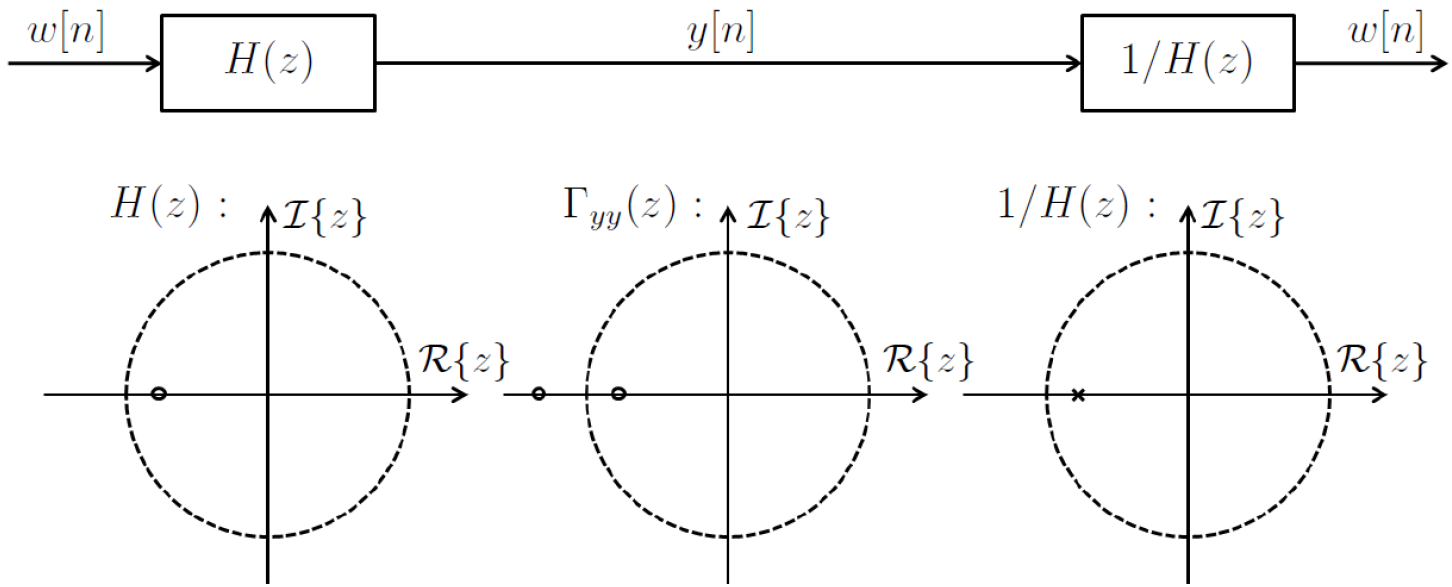
\includegraphics[width=0.7\textwidth]{../fig/beispiel_ma_modell}
\end{center}
\newpage

%===============================================================================
\subsection{Autoregressive model (AR)}
Oft ist ein AR-Modell sinnvoller als MA. Die Zufallssequenz wird durch einen All-pole Filter generiert:
\[ y[n] = w[n] - \sum_{k=1}^{N}a_k\cdot y[n-k] \]
Es gilt:
\begin{itemize}[noitemsep,topsep=3pt]
	\item $H(z)$ = kausales Filter \emph{nur} mit Polstellen
	\item $1/H(z)$ = kausales Filter \emph{nur} mit Nullstellen
\end{itemize}
Berechnung der Koeffizienten bei gegebener Autokorrelation $\gamma_{yy}$:
\[ \gamma_{yy}[m] = \left\lbrace \begin{matrix}
	-\sum_{k=1}^{N}a_k\cdot\gamma_{yy}[m-k] & \textrm{if } m>0\\
	\sigma_0^2-\sum_{k=1}^{N}a_k\cdot\gamma_{yy}[m-k] & \textrm{if } m =0\\
	\gamma_{yy}^*[-m]	& \textrm{if } m < 0
\end{matrix}\right. \]
\textbf{Yule-Walker Gleichungen:} Das Gleichungssystem in Matrizenform lautet:
\[ \begin{bmatrix}
	\gamma_{yy}[0] & \gamma_{yy}[-1] & \ldots & \gamma_{yy}[-N]\\
	\gamma_{yy}[1] & \gamma_{yy}[0] & \ldots & \gamma_{yy}[-N+1]\\
	\vdots & \vdots & & \vdots\\
	\gamma_{yy}[N] & \gamma_{yy}[N-1] & \ldots & \gamma_{yy}[0]
\end{bmatrix} \cdot \begin{bmatrix}
	1 \\ a_1 \\ \vdots \\ a_N \end{bmatrix} = \begin{bmatrix}
	\sigma_w^2 \\ 0 \\ \vdots \\ 0 \end{bmatrix} \]  
~\\
\textbf{Achtung:} Durch falsche Parametrisierung kann ein AR-Modell instabil werden!
	
%===============================================================================
\subsection{ARMA model}
Ist die Zusammensetzung des MA und AR Models. Dabei sind die Ordnungen der
Polynomen $B(z)$ und $A(z)$ 1 oder höher. Somit hat der Pol-Nullstellenplan
Nullen und Pole. Dieser ist allerdings geeigneter als die Spezialfälle MA und
AR, da weniger Koeffizienten für ein gutes Model benötigt werden.

%===============================================================================
\section{Abschätzung der Spektrums-Dichtefunktion}
Gegeben sei eine Messserie $x[0], x[1],...,x[N-1]$ eines stationären stochastischen Prozesses.
\subsection{Parameterlose Methode}
Nachteil: Für jedes $\Omega_0$ weisst die Schätzung $\hat{\Gamma}_{xx}(\Omega_0)$ eine grosse Varianz auf.
Sie verändert sich auch nicht mit höherer Anzahl Samples.\\\\
Alternativ kann zuerst die Autokorrelation, daraus mittels Wiener-Khinchin-Theorem das Spektrum
ermittelt werden. Es existieren die folgenden beiden Methoden:
\begin{itemize}[noitemsep,topsep=3pt]
	\item \emph{Biased} autocorrelation estimator:  \\
								$\hspace{10mm} \hat{\gamma}_{xx}[m]=\frac{1}{N} \cdot \sum_{n=0}^{N-m-1} x^*[n]\cdot x[n+m] 
								\qquad \text{, für } m \text{ zwischen 0 und } N-1$
	\item \emph{Unbiased} autocorrelation estimator:\\
								$\hspace{10mm} \hat{\gamma}_{xx}[m]=\frac{1}{N-m} \cdot \sum_{n=0}^{N-m-1} x^*[n]\cdot x[n+m] 
								\qquad \text{, für } m \text{ zwischen 0 und } N-1$
\end{itemize}
Das Problem bei der "'unbiased"' Variante ist, dass mit grösserem $m$ der Bruch immer fragiler wird.
Die "'biased"' Methode erzielt meistens bessere Resultate aufgrund der Fehlerreduktion durch die höhere
Anzahl an Samples. 
\subsection{Parameterbehaftete Methode}
Falls Informationen über die Struktur der Rauschquelle vorhanden sind, 
können diese bei der Modellierung helfen. Auch ohne Informationen ist es 
aber möglich, mit einer parametrischen Methode ein passendes Modell zu 
ermitteln. \\\\
ARMA-Modelle sind weit verbreitet, da sie mit den Parametern fein angepasst werden können. 
Für Spektren mit Spitzen passt ein AR-Modell besser als ein MA-Modell.